%! Licence = CC BY-NC-SA 4.0

%! Author = gianfluetsch
%! Date = 22. Jan 2022
%! Project = icth_summary

\section{Leitungscodierung}
\subsection{R}
\subsubsection{A}
\textbf{RS232}\\
Wie viele Datenbits könnte man in einem Zeichen haben, damit das letzte Bit gerade noch innerhalb der Bitdauer abgetastet wird, wenn der Empfänger eine um 5\% langsamere Taktfrequenz besitzt als der Sender? Veranschaulichen sie die Situation durch eine Skizze.
\begin{center}
    \vspace{-8pt}
    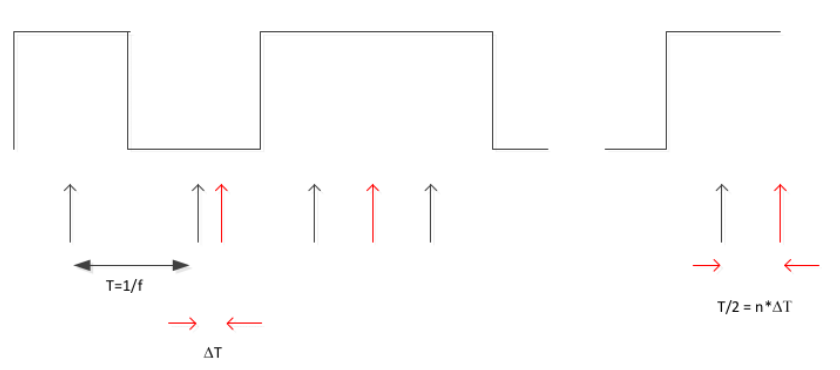
\includegraphics[width=.6\linewidth]{./06-leitungscodierung/aufgabe_w09}
    \vspace{-8pt}
\end{center}

Mit jedem Bit verschiebt sich der Takt um ein $\Delta T$ von\\
$\Delta T=\frac{1}{1-\delta }T-T=\frac{\delta}{1-\delta}T$\\
Der Grenzfall ist erreicht, falls $n*\Delta T = \frac{1}{2}T:$\\
$n*\Delta T = \frac{1}{2}T \rightarrow n\frac{\delta}{1-\delta}T=\frac{1}{2}T$\\
$n=\frac{1-\delta}{2\delta}=\frac{1-0.05}{2*0.05}=9.5$\\
D.h. nach dem ersten, also 0-ten Bit, können noch 9 Bit abgetastet werden.\\

\textbf{Codierung}\\
\begin{center}
    \vspace{-8pt}
    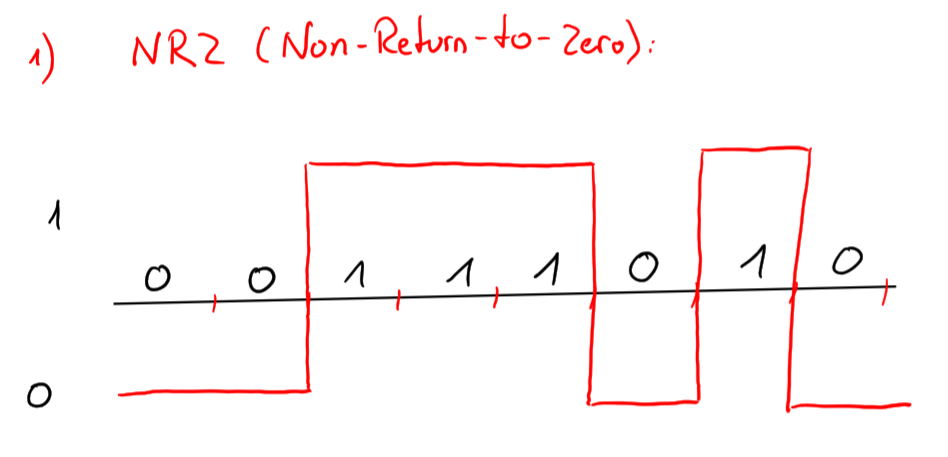
\includegraphics[width=.8\linewidth]{./06-leitungscodierung/aufgabe_w09_2}
    \vspace{-8pt}
\end{center}
\begin{center}
    \vspace{-8pt}
    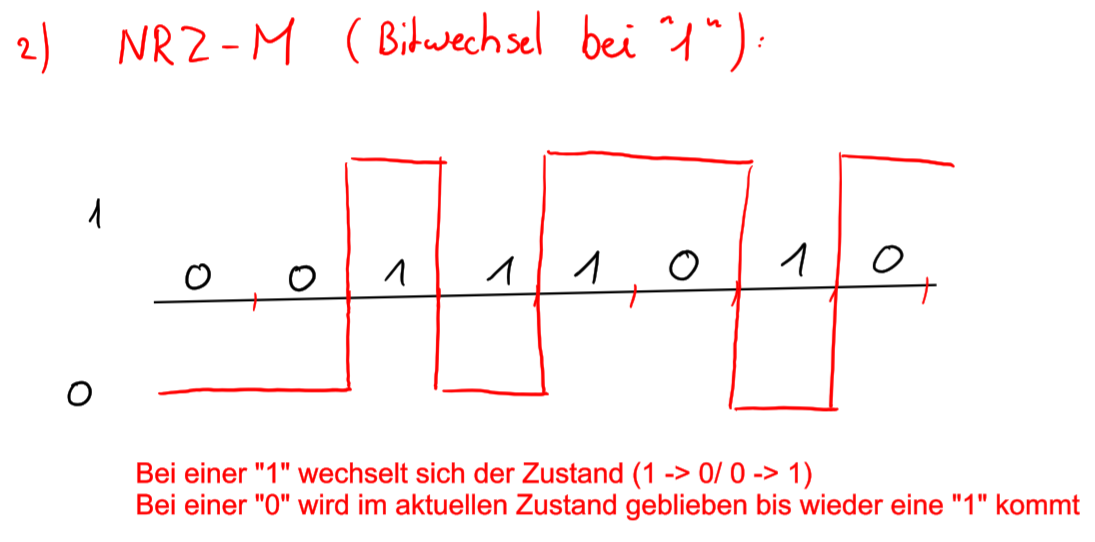
\includegraphics[width=.8\linewidth]{./06-leitungscodierung/aufgabe_w09_3}
    \vspace{-8pt}
\end{center}
\begin{center}
    \vspace{-8pt}
    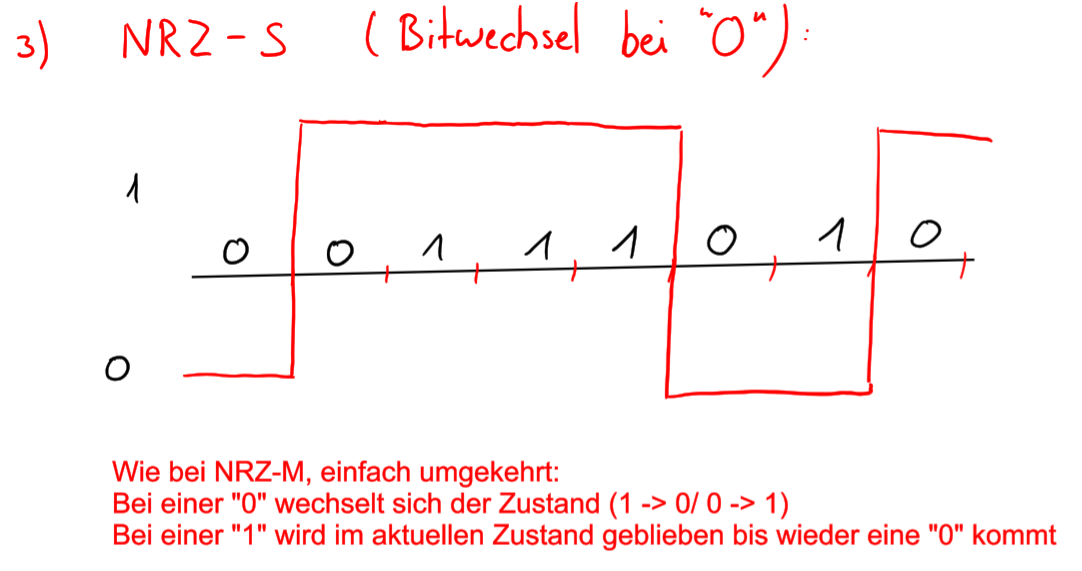
\includegraphics[width=.8\linewidth]{./06-leitungscodierung/aufgabe_w09_4}
    \vspace{-8pt}
\end{center}
\begin{center}
    \vspace{-8pt}
    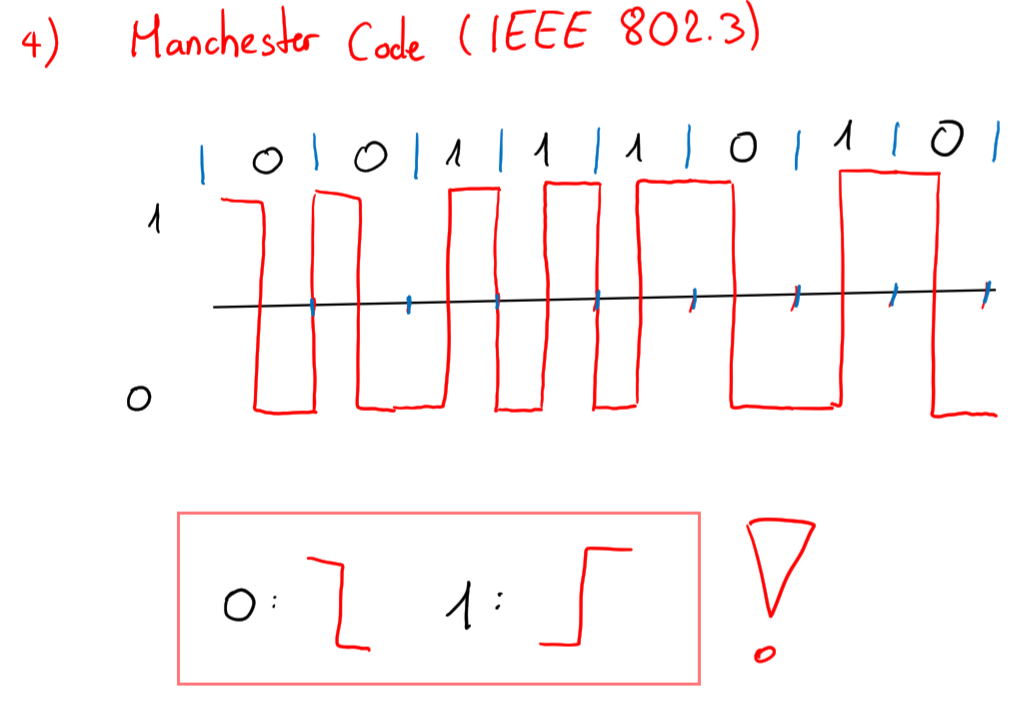
\includegraphics[width=.8\linewidth]{./06-leitungscodierung/aufgabe_w09_5}
    \vspace{-8pt}
\end{center}


\subsubsection{B}
Ein NRZ Signal hat den unten aufgezeichneten Signalverlauf. Skizzieren Sie den entsprechenden Signalverlauf sowohl für den Manchester Code als auch für den AMI-Code.
\begin{center}
    \vspace{-8pt}
    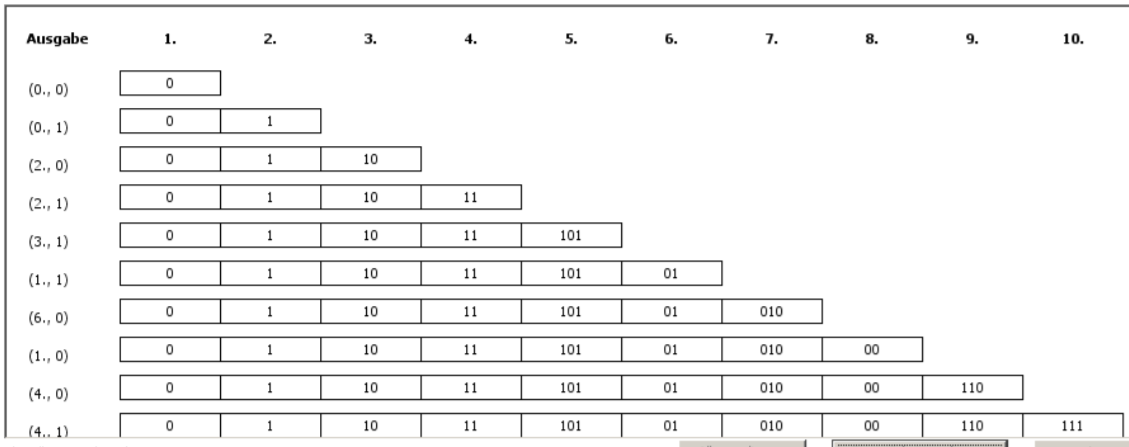
\includegraphics[width=.8\linewidth]{./06-leitungscodierung/fs2009}
    \vspace{-8pt}
\end{center}

\textbf{Vergleichen Sie die drei Codierungsarten anhand der oben gegebenen und der erstellten Codierungen.}\\
Lange 0-Folgen werden beim AMI Code zu einem Problem wegen der Phasen und Taktrückgewinnung. NRZ hat dieselben Probleme der Phasen- und Taktrückgewinnung bei
langen 0 oder 1 Folgen. Der Manchestercode weist bei jedem Bit einen Pegelwechsel auf.

\subsection{S}

\subsubsection{A}
In der untentstehenden Grafik wird ein binäres Datensignal mittels einer Leitungscodes über einen Kommunikationskanal übertragen:
\begin{center}
    \vspace{-8pt}
    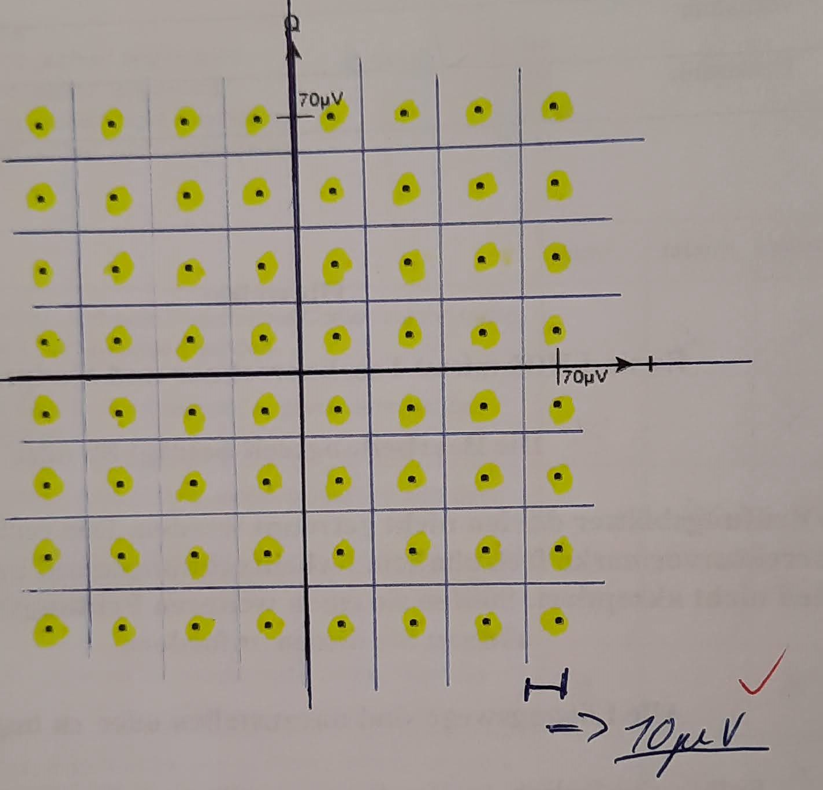
\includegraphics[width=.9\linewidth]{./06-leitungscodierung/hs2020-2}
    \vspace{-8pt}
\end{center}

\textbf{Um welchen Leitungscode handelt es sich?}\\
Bipolarer NRZ (Non Return to Zero) Code.\\

\textbf{Ist der Leitungscode bei allen möglichen Datensequenzen mittelwertfrei?}\\
$\rightarrow$ nicht mittelwertfrei, da lange '0'-Folgen entweder einen positiven oder negativen DC-Offset bewirken.\\

\textbf{Bei welchen Datensequenzen könnte beim Empfänger der Takt verloren gehen?}\\
Der Takt kann bei langen '0'-Folgen verloren gehen, da keine Pegelwechsel stattfinden.\\

\textbf{Mit welcher Zusatzmassnahme könnte die Mittelwertfreiheit und die Taktextraktion mit hoher Wahrscheinlichkeit garantiert werden?}\\
Durch Scramkeln der Datensequenz vor der Leitungscodierung könnte die Mittelwertfreiheit und die Taktextraktion mit hoher Wahrscheinlichkeit garantiert werden.

\subsubsection{B}
Eine Datenquelle sendet dauernd die Nullsequenz $'... 0 0 0 0 0 0 ...'$. Kreuzen Sie an, ob die unten aufgeführten Leitungscodes für diese Sequenz annähernd gleichspannungsfrei sind, respektive ob genügend Pegelwechsel für eine Taktrückgewinnung vorhanden sind.
\begin{center}
    \vspace{-8pt}
    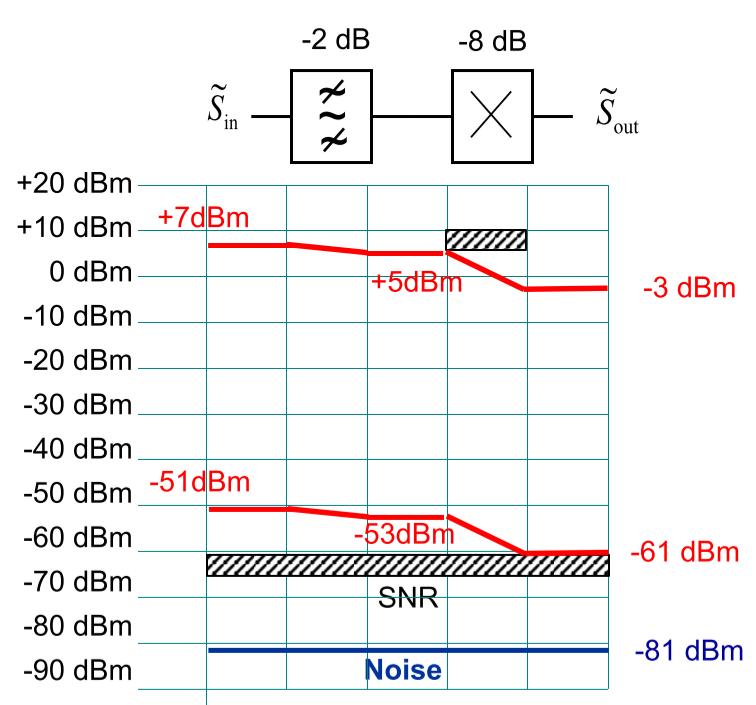
\includegraphics[width=.9\linewidth]{./06-leitungscodierung/hs2018}
    \vspace{-8pt}
\end{center}

\subsubsection{C}
Eine Datenquelle sendet dauernd die Einersequenz $'....1 1 1 1 1 1 ...'$. Kreuzen Sie an, ob die unten aufgeführten Leitungscodes für diese Sequenz annähernd gleichspannungsfrei sind, res-
pektive ob genügend Pegelwechsel für eine Taktrückgewinnung vorhanden sind.
\begin{center}
    \vspace{-8pt}
    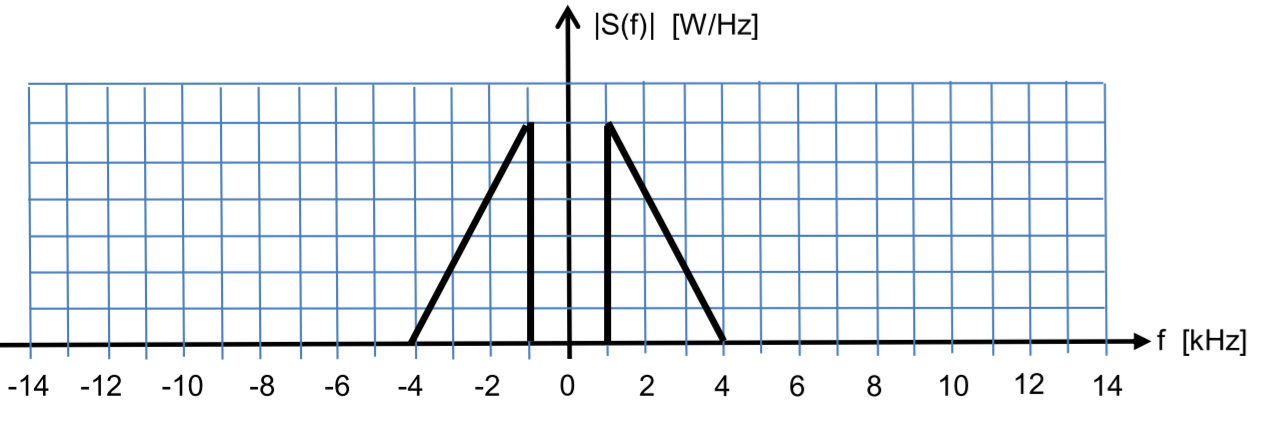
\includegraphics[width=.9\linewidth]{./06-leitungscodierung/hs2016}
    \vspace{-8pt}
\end{center}
